Este apêndice apresenta os equipamentos usados no desenvolvimento do gerador e nos ensaios em bancada.

A placa de desenvolvimento Terasic DE2-115 (Figura~\ref{fig:inst_de2115}) traz o \ac{fpga} Cyclone IV E EP4CE115F29C7 e recebeu todo o projeto digital. Dela foram usados o oscilador de 50~MHz, o botão KEY[0], dois \eng{LEDs}, o conector de expansão ligado à placa analógica e o USB-Blaster embutido, para a gravação do \ac{fpga} e o controle pelo Virtual \ac{jtag}.

\begin{figure}
	\caption{Placa de desenvolvimento Terasic DE2-115.}
	\label{fig:inst_de2115}
	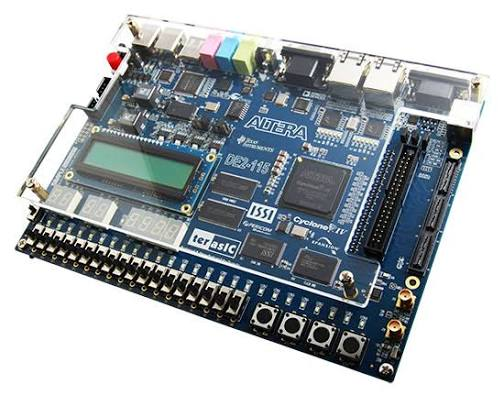
\includegraphics[width=0.55\textwidth]{./figuras/inst_de2-115}
	\legend{Fonte~---~Terasic.}
\end{figure}

O osciloscópio digital Tektronix TBS1102B, de dois canais, 100~MHz e 2~GS/s (Figura~\ref{fig:inst_tbs1102b}), fez todas as medidas de bancada da Seção~\ref{sec:bancada}, cujas telas estão no Apêndice~\ref{ap:osciloscopio}.

\begin{figure}
	\caption{Osciloscópio digital Tektronix TBS1102B.}
	\label{fig:inst_tbs1102b}
	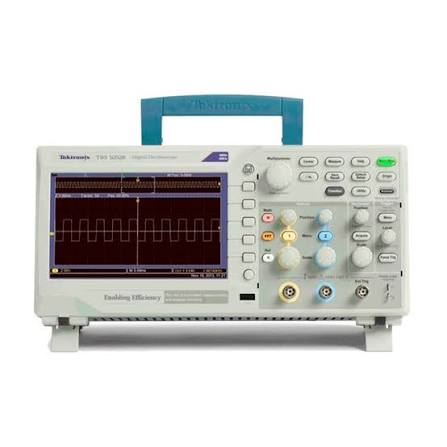
\includegraphics[width=0.45\textwidth]{./figuras/inst_tbs1102b}
	\legend{Fonte~---~Tektronix.}
\end{figure}

O multímetro digital Minipa ET-2042F (Figura~\ref{fig:inst_et2042f}) foi usado para conferir as tensões de alimentação da placa analógica e a continuidade das linhas do barramento do \acs{dac}.

\begin{figure}
	\caption{Multímetro digital Minipa ET-2042F.}
	\label{fig:inst_et2042f}
	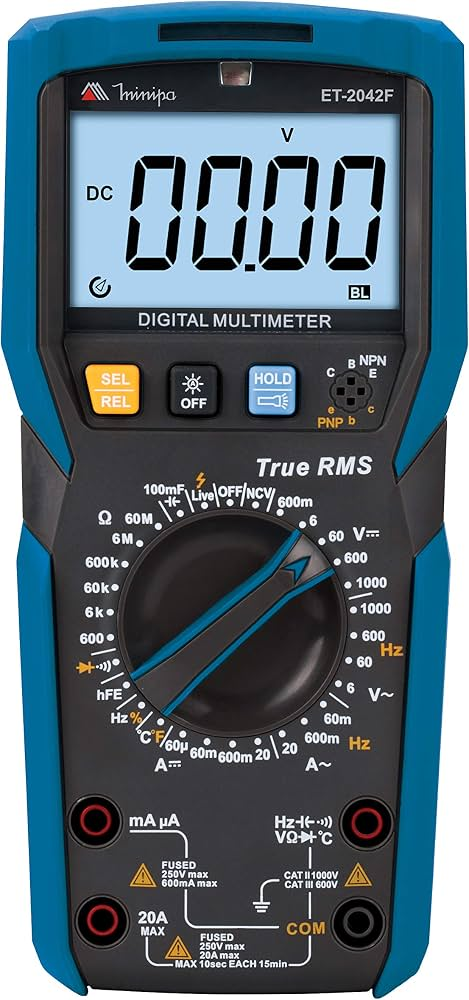
\includegraphics[width=0.25\textwidth]{./figuras/inst_et-2042f}
	\legend{Fonte~---~Minipa.}
\end{figure}

A fonte de alimentação de bancada ICEL Manaus PS-5000, de dois canais de 0 a 32~V e 0 a 3~A (Figura~\ref{fig:inst_ps5000}), alimentou a placa analógica.

\begin{figure}
	\caption{Fonte de alimentação ICEL Manaus PS-5000.}
	\label{fig:inst_ps5000}
	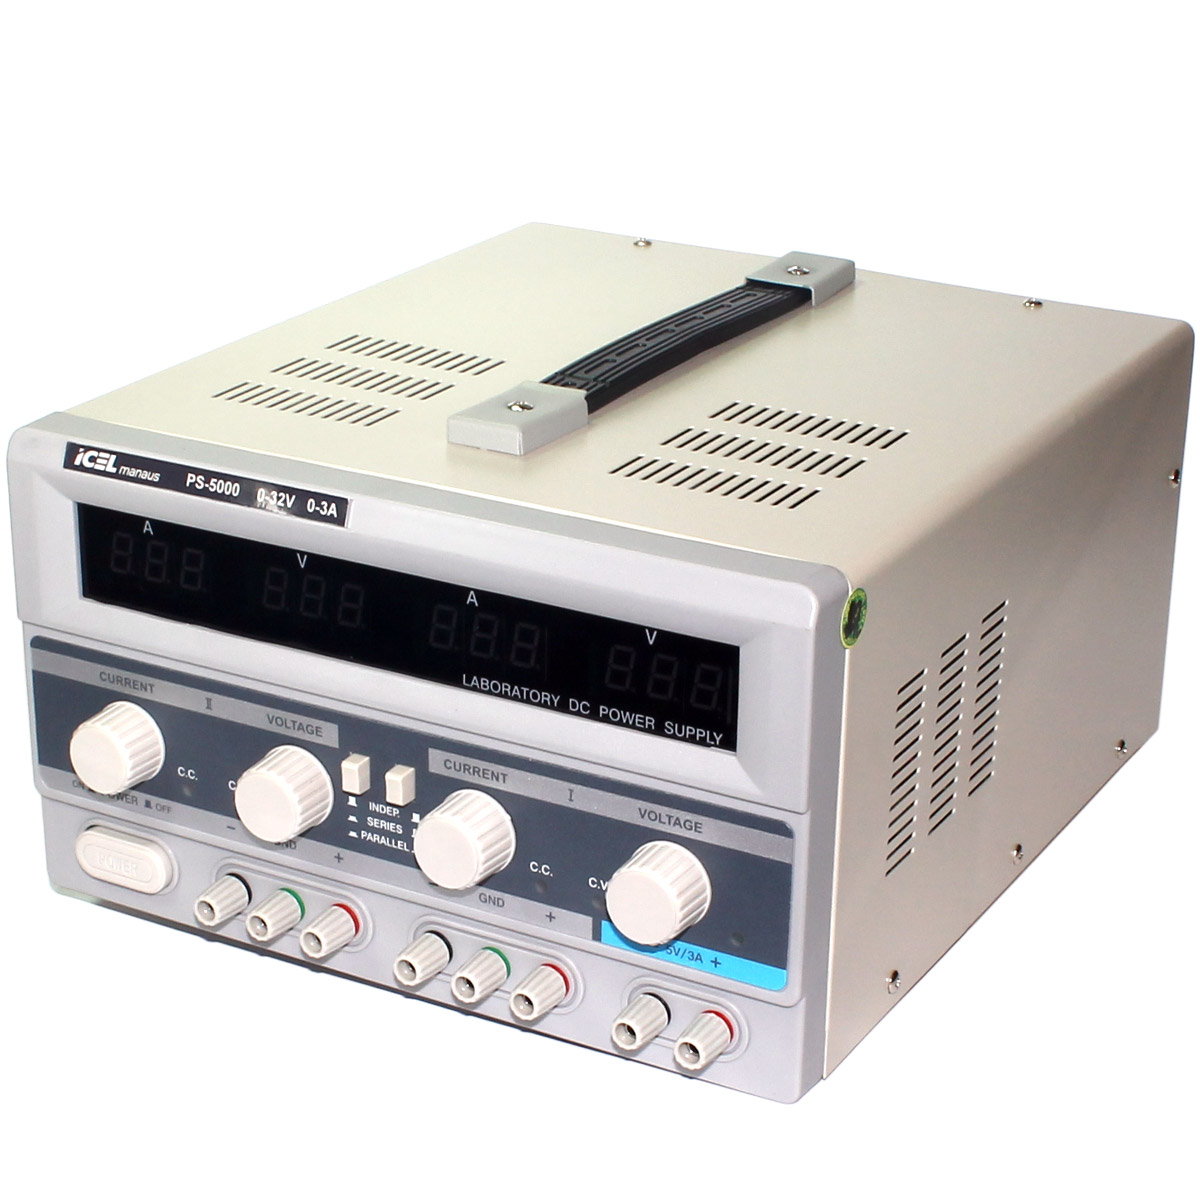
\includegraphics[width=0.45\textwidth]{./figuras/inst_ps-5000}
	\legend{Fonte~---~ICEL Manaus.}
\end{figure}

O \eng{pendrive} SanDisk Cruzer Blade de 16~GB (Figura~\ref{fig:inst_cruzer}) guardou as telas e os dados salvos pelo osciloscópio.

\begin{figure}
	\caption{\eng{Pendrive} SanDisk Cruzer Blade de 16~GB.}
	\label{fig:inst_cruzer}
	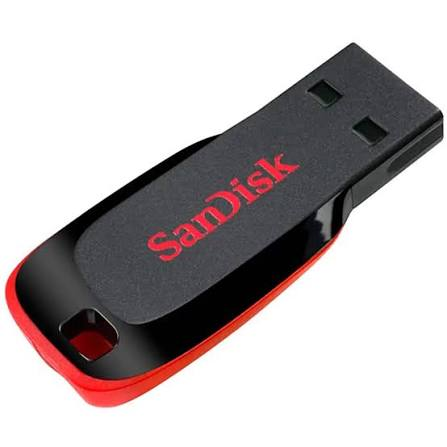
\includegraphics[width=0.35\textwidth]{./figuras/inst_cruzer_blade}
	\legend{Fonte~---~SanDisk.}
\end{figure}
